\documentclass{article}
\usepackage[utf8]{inputenc}
\usepackage[spanish,mexico]{babel}
\usepackage[margin=2.3cm]{geometry}
\usepackage{graphicx}
\usepackage[export]{adjustbox}
\usepackage{caption}
\usepackage{subcaption}
\usepackage{fancyhdr}
\usepackage{lipsum}
\usepackage{float}
\usepackage{upgreek}
\usepackage{physics}
\usepackage{cancel}
\usepackage{amsfonts, amsthm}
\usepackage{amssymb, latexsym, amsmath}
\usepackage{ textcomp }
%%\usepackage{graphicx}
%%\usepackage{subcaption}
\usepackage{url}

% Evitar sangrías
\setlength{\parindent}{0cm}

% Código
\newcommand{\code}[1]{\textcolor{white!25!black}{\texttt{#1}}}

% ASA
\usepackage{tree-dvips}
\usepackage{qtree}
\usepackage[linguistics]{forest}

% Letter colors.
\usepackage{xcolor}
%\usepackage[usenames,dvipsnames,svgnames,table]{xcolor}

%%Tablas con color
\usepackage{xcolor, colortbl}
\usepackage{array, multirow, multicol}
\cellcolor[modelo color]{color}

\pagestyle{fancy}
\fancyhf{}

\title{Facultad de Ciencias, UNAM}
\date{\today}

\begin{document}

\thispagestyle{empty}
	
	\begin{figure}[ht]
	   \minipage{0.76\textwidth}
			
\includegraphics[width=4cm]{Logo_UNAM.png}
			\label{EscudoUNAM}
	   \endminipage
	   \minipage{0.32\textwidth}
			
\includegraphics[height = 4.9cm ,width=4cm]{Logo_FC.png}
			\label{EscudoFC}
		\endminipage
	\end{figure}
	
	\begin{center}
	\vspace{0.8cm}
	\LARGE
	UNIVERSIDAD NACIONAL AUTÓNOMA DE MÉXICO 
	
	\vspace{0.7cm}
	\LARGE
	FACULTAD DE CIENCIAS
	
	\vspace{0.8 cm}	
	\Large
	\textbf{Tarea 2}

	\vspace{0.8 cm}
	\normalsize	
	INTEGRANTES \\
	\vspace{.2cm}
	\large
	\textbf{Torres Valencia Kevin Jair - \texttt{318331818}}\\
	\textbf{Aguilera Moreno Adrián - \texttt{421005200}}\\
	\textbf{Rivera Silva Marco Antonio - \texttt{318183583}}\\
	
	\vspace{1 cm}
	\normalsize	
	PROFESORA \\
	\vspace{.2cm}
	\large
	\textbf{Karla Ramírez Pulido}
	
	\vspace{1 cm}
	AYUDANTES \\
	\vspace{.2cm}
	\large
	\textbf{Alan Alexis Martínez López}\\
	\textbf{Manuel Ignacio Castillo López}\\
	\textbf{Alejandra Cervera Taboada}
	\vspace{1.3cm}
	
	\normalsize	
	ASIGNATURA \\
	\vspace{.2cm}
	\large
	\textbf{Lenguajes de Programación}
	
	\vspace{1 cm}
	\today
	\end{center}
	
	\newpage
	\textbf{\textcolor{blue}{1.}} \Large
Currifica cada uno de los siguientes términos.

\renewcommand{\theenumi}{\alph{enumi}}
\begin{itemize}

\item $\lambda abc.abc$.\\
\textbf{Solución:}
$\lambda a. \lambda b. \lambda c. abc$
%%%%%%%%%%%%%%%%%%%%%%%%%%%%%%%%%%%%%%%%%%%%%%
\item $\lambda abc. \lambda cde.acbdce$.\\
\textbf{Solución:}
$\lambda a.\lambda b.\lambda c.\lambda c.\lambda d.\lambda e.acbdce$
%%%%%%%%%%%%%%%%%%%%%%%%%%%%%%%%%%%%%%%%%%%%%%
\item $(\lambda d.(\lambda de.e) (\lambda fc.c)) (\lambda ab.b)$.\\
\textbf{Solución:}
$(\lambda d.(\lambda d.\lambda e.e)(\lambda f.\lambda c.c))(\lambda a.\lambda b.b)$
\end{itemize}

        \vspace*{0.5cm}
%%%%%%%%%%%%%%%%%%%%%%%%%%%%% Inciso 1A:
$a$) $\{-\; 30\; \{+\; 15\; \{+\; 40\; 5\;\}\; \}\; \}$

\hspace*{0.3cm} La representación del \code{ASA}
para la expresión anterior, tiene la forma siguiente
\begin{center}
  \begin{forest}
    [$-$ [$30$] [$+$ [$15$] [$+$ [$40$] [$5$]]]]
  \end{forest}
\end{center}

        \vspace*{0.5cm}
%%%%%%%%%%%%%%%%%%%%%%%%%%%%% Inciso 1A:
$b$) $\{-\; 30\; \{+\; 300\; \{+\; 40\; \}\; \}\; \}$

\hspace*{0.3cm} En este caso, particular,

        \vspace*{0.3cm}
%%%%%%%%%%%%%%%%%%%%%%%%%%%%% Inciso 1C:
$c$) $\{$ \code{with} $\{a\;\: 3\}$                                 \newline
\hspace*{0.7cm} $\{$ \code{with} $\{b\;\: \{-\;\: a\;\: a\}\: \}$   \newline
\hspace*{1.2cm} $\{+\;\: a\;\: \{-\;\: b\;\:\:\; 8\;\:\}\:\; \}$    \newline

\hspace*{0.3cm} La representación del \code{ASA} para la anterior expresión
es
\begin{center}
  \begin{forest}
    [\code{with} [$a$ [$3$]] [\code{with} [$b$ [$-$ [$a$] [$a$]]] [$+$ [$a$] [$-$ [$b$] [$8$]]]]]
  \end{forest}
\end{center}

	\textbf{\textcolor{blue}{2.}} \Large
Aplica $\alpha$-conversiones en cada expresión
para cambiar los términos de las variables de ligado.
\begin{enumerate}[a)]
%%%%%%%%%%%%%%%%%%%%%%%%      Inciso a    %%%%%%%%%%%%%%%%%%%%%%%%%%%%
    \item $\lambda a.\lambda b.(\lambda a.b \; \lambda b.a)$
%%%%%%%%%%%%%%%%%%%%%%%%      Inciso b    %%%%%%%%%%%%%%%%%%%%%%%%%%%%
    \item $\lambda a.(a(\lambda b.(\lambda a.a\; b)a))$
%%%%%%%%%%%%%%%%%%%%%%%%      Inciso c    %%%%%%%%%%%%%%%%%%%%%%%%%%%%
    \item $\lambda x.(\lambda y.x\; \lambda y(\lambda x.x \; y))$
\end{enumerate}

        \vspace*{0.3cm}
%%%%%%%%%%%%%%%%%%%%%%%%%%%%% Inciso 2A:
$a$) $e\: =\: \{+\: a\:\; \{+\: b\:\; \{-\: 32\:\; 57\: \}\: \}\: \}$ \newline
\hspace*{0.5cm} \code{(subst (parse e) '$a$ (add (num 3) (num 4)))}   \newline

\hspace*{0.3cm} Primero demos la representación abstracta de la expresión
anterior, esta es
\begin{center}
  \begin{forest}
    [$+$ [$a$] [$+$ [$b$] [$-$ [$32$] [$57$]]]]
  \end{forest}
\end{center}

\hspace*{0.3cm} Luego apliquemos la instrucción \code{parse} a la expresión
\code{e}, esto es
\begin{eqnarray*}
  \text{\code{(parse e)}} &=& \code{(add (parse($a$)) (parse($\{+\; b\; \{-\; 35\;\; 57\}\}$)))}\\
  &=& \code{(add (id '$a$) (add (parse($b$)) (parse($\{-\; 35\;\; 57\}$))))}\\
  &=& \code{(add (id '$a$) (add (id '$b$) (sub (parse($35$)) (parse($57$)))))}\\
  &=& \code{(add (id '$a$) (add (id '$b$) (sub (num $35$) (num $57$))))}\\
  &=& \code{e'}
\end{eqnarray*}
ahora, apliquemos la instrucción \code{subst} a \code{e'} y los valores indicados,
esto es

\begin{center}
  \fbox{
    \begin{minipage}[b][1\height]%
      [t]{0.867\textwidth}
      \textbf{Obs.} Por simplicidad, asumimos que
      \begin{center}
        \code{subst(e') = (subst (e') 'a (add (num 3) (num 4)))}
      \end{center}
  \end{minipage}}
\end{center}
\begin{eqnarray*}
  \code{subst (e')} &=& \code{(add (subst (id '$a$))
    (subst ((add (id '$b$) (sub (num $35$) (num $57$))))))}\\
  &=& \code{(add (add (num 3) (num 4))
    ((add (subst (id '$b$)) (subst (sub (num $35$) (num $57$))))))}\\
  &=& \code{(add (add (num 3) (num 4))
    ((add  (id '$b$)  (sub (subst (num $35$)) (subst (num $57$))))))}\\
    &=& \code{(add (add (num 3) (num 4))
    ((add  (id '$b$)  (sub (num $35$) (num $57$)))))}
\end{eqnarray*}


        \vspace*{0.3cm}
%%%%%%%%%%%%%%%%%%%%%%%%%%%%% Inciso 2B:
$b$) $e\: =\: \{\; \code{with } \{y\;\; \{-\; 30\; \{-\; y\;\; z\; \}\; \} $ \newline
\hspace*{1.5cm} $\{-\; 30\; \{+\; y\;\; z\; \}\; \}$                         \newline
\hspace*{0.3cm} \code{(subst (parse e) 'y (id 'w))}                          \newline

\hspace*{0.3cm} Primero veamos como esta construida la representación abstracta de
la expresión anterior, esta es
\begin{center}
  \begin{forest}
    [\code{with} [$y$ [$-$ [$30$] [$+$ [$y$] [$z$]]]] [$-$ [$30$] [$+$ [$y$] [$z$]]]]
  \end{forest}
\end{center}

Luego, apliquemos la instrucción \code{parse} a la expresión
\code{e}, esto es
\begin{eqnarray*}
  \code{(parse e)} &=& \code{(with (parse $\{\; y\; \{-\; 30\; \{-\; y\; z\; \}\}$)
  (parse $\{-\; 30\; \{+\; y\; z\; \}\}$))}\\
  &=& \code{(with (((parse $y$) (parse $\{-\; 30\; \{-\; y\; z\; \}\}$))))}\\
  & & \code{(sub (parse $30$) (parse $\{+\; y\; z\; \}$)))}\\
  &=& \code{(with ((id '$y$) (sub (parse $30$) (parse $\{-\; y\; z\; \}\}$))))}\\
  & & \code{(sub (num $30$) (add (parse $y$) (parse $z$))))}\\
  &=& \code{(with ((id '$y$) (sub (num $30$) (sub (parse $y$) (parse $z$)))))}\\
  &=& \code{(sub (num $30$) (add (id '$y$) (id '$z$))))}\\
  &=& \code{(with ((id '$y$) (sub (num $30$) (sub (id '$y$) (id '$z$)))))}\\
  &=& \code{(sub (num $30$) (add (id '$y$) (id '$z$))))}\\
  &=& \code{e'}
\end{eqnarray*}

Ahora, apliquemos la instrucción \code{subst} a \code{e'} y los valores indicados,
esto es (se obvia la observación anterior)

\begin{eqnarray*}
  \code{(subst e)} &=& \code{(subst (with ((id '$y$) (sub (num $30$) (sub (id '$y$) (id '$z$)))))}\\
  & & \code{(sub (num $30$) (add (id '$y$) (id '$z$)))))}\\
  &=& \code{(with ((id '$y$) (subst (sub (num $30$) (sub (id '$y$) (id '$z$))))))}\\
  & & \code{(sub (num $30$) (add (id '$y$) (id '$z$)))))}\\
  &=& \code{(with ((id '$y$) (sub (subst (num $30$)) (subst (sub (id '$y$) (id '$z$))))))}\\
  & & \code{(sub (num $30$) (add (id '$y$) (id '$z$)))))}\\
  &=& \code{(with ((id '$y$) (sub (num $30$) (sub (subst (id '$y$)) (subst (id '$z$))))))}\\
  & & \code{(sub (num $30$) (add (id '$y$) (id '$z$)))))}\\
  &=& \code{(with ((id '$y$) (sub (num $30$) (sub (id '$w$) (id '$z$)))))}\\
  & & \code{(sub (num $30$) (add (id '$y$) (id '$z$)))))}\\.
\end{eqnarray*}

        \vspace*{0.3cm}
%%%%%%%%%%%%%%%%%%%%%%%%%%%%% Inciso 2C:
$c$) $e\: =\: \{\; \code{with} \{y\;\; \{-\; 30\; \{-\; y\;\; z\; \}\; \} $ \newline
\hspace*{1.5cm} $\{-\; 30\; \{+\; y\;\; z\; \}\; \}$                       \newline
\hspace*{0.3cm} \code{(subst (parse e) 'z (id 'v))}

        \textbf{\textcolor{blue}{3.}} \Large
Aplica $\beta$-reducciones a las siguientes expresiones
para llegar a una Forma Normal, en caso de que no se pueda justifica. Además indica
en cada paso el reducto y el redex.\\

$l\;=_{def} \lambda a.a$\\
$K\;=_{def} \lambda a.\lambda b.a$\\
$S\;=_{def} \lambda a.\lambda b.\lambda a.ac(bc)$\\
$\Omega\; =_{def} (\lambda a.aa) (\lambda a.aa)$

\begin{enumerate}[a)]
%%%%%%%%%%%%%%%%%%%%%%%%      Inciso a    %%%%%%%%%%%%%%%%%%%%%%%%%%%%
    \item $\lambda a.aK\Omega$

    \textbf{Solución:}
    \begin{eqnarray*}
        \lambda_a .aK\Omega &\equiv& \lambda_a .a
        (\lambda_a . \lambda_b . a)
        ((\underbrace{\lambda a.aa}_{Redex}) (\lambda a.aa))\\
        &\rightarrow_{\beta}&
        \lambda_a .a (\lambda_a .a)(\underbrace{(\lambda a.aa) (\lambda a.aa)}_{Reducto}).
    \end{eqnarray*}
    Esta $\lambda$-función diverge, como se puede observar en la $\beta$-reducción anterior.
%%%%%%%%%%%%%%%%%%%%%%%%      Inciso b    %%%%%%%%%%%%%%%%%%%%%%%%%%%%
    \item $(\lambda a.a(ll))c$

    \textbf{Solución:}
    \begin{eqnarray*}
        (\lambda_a .a(ll))c &\equiv& \lambda_a . a((\underbrace{\lambda_a .a}_{Redex})
        (\lambda_a .a))c\\
        &\rightarrow_{\beta}& \lambda_a .
        a(\underbrace{\lambda_a .a}_{\text{Reducto y Redex}})c\\
        &\rightarrow_{\beta}& \underbrace{\lambda_a . a}_{Redex} \underbrace{c}_{Reducto}\\
        &\rightarrow_{\beta}& \underbrace{c}_{Reducto}.
    \end{eqnarray*}
%%%%%%%%%%%%%%%%%%%%%%%%      Inciso c    %%%%%%%%%%%%%%%%%%%%%%%%%%%%
    \item $(\lambda d.\lambda e.(\lambda f.f(\lambda a.ad))e)b(\lambda c.\lambda b.cb)$

    \textbf{Solución:}
    \begin{eqnarray*}
        (\lambda_d .\lambda_e .(\underbrace{\lambda_f .f}_{Redex}
        (\lambda_a .ad))e)b(\lambda_c .\lambda_b .cb)
        &\rightarrow_\beta&
        (\lambda_d .\lambda_e
        .(\underbrace{\overbrace{\lambda_a .a}^{Redex}d}_{Reducto})e)
        b(\lambda_c .\lambda_b .cb)\\
        &\rightarrow_\beta& (\lambda_d .\overbrace{\lambda_e .\underbrace{e}_{Reducto}}^{Redex}
        (d) b(\lambda_c .\lambda_b .cb)\\
        &\rightarrow_\beta& (\overbrace{\lambda_d .\underbrace{d}_{Reducto}}^{Redex}
        (b)(\lambda_c .\lambda_b .cb)\\
        &\rightarrow_\beta& \underbrace{b}_{Reducto}
        ((\underbrace{\lambda_c .\lambda_b .c}_{Redex})b)\\
        &\rightarrow_\beta& b \underbrace{\lambda_b . b}_{Reducto}.
    \end{eqnarray*}
\end{enumerate}

	\textbf{\textcolor{blue}{4.}} \Large
Usando recursión de cola optimiza la función del Ejercicio 2. Toda función auxiliar ocupada
debe ser optimizada.\\

	\Large\textbf{\textcolor{blue}{5.  *Punto extra*}} 
Observa la siguiente función del lenguaje de programación \code{Racket}

\begin{lstlisting}
(let ([sum (lambda (n) (if (zero? n) 0 (+ n (sum (sub1 n))))))])
      (sum 5))
\end{lstlisting}

\begin{enumerate}[a.]
%%%%%%%%%%%%%%%%%%%%%%%%%%%%%      Inciso A        %%%%%%%%%%%%%%%%%%%%%%%%%%%%%%%%%
\item Prueba la expresión en el intérprete de \code{Racket} y con base en la respuesta 
obtenida, explica el proceso que siguió el intérprete para llegar a ésta. Anexa una 
captura de pantalla del intérprete de \code{Racket} al probar la expresión.

\begin{figure}[h]
  \centering
  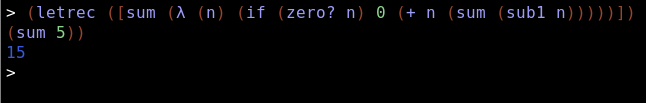
\includegraphics[scale=0.5]{./Sum.png}
  \caption{Ejecución de la función dada.}
\end{figure}

\begin{lstlisting}
> (let ([sum (lambda (n) (if (zero? n) 0 (+ n (sum (sub1 n))))))])
      (sum 5))
= (+ 5 (sum 4))
= (+ 5 (+ 4 (sum 3)))
= (+ 5 (+ 4 (+ 3 (sum 2))))
= (+ 5 (+ 4 (+ 3 (+ 2 (sum 1)))))
= (+ 5 (+ 4 (+ 3 (+ 2 (+ 1 0)))))
= (+ 5 (+ 4 (+ 3 (+ 2 (1)))))
= (+ 5 (+ 4 (+ 3 (3))))
= (+ 5 (+ 4 (+ 6)))
= (+ 5 (10))
= 15
\end{lstlisting}
%%%%%%%%%%%%%%%%%%%%%%%%%%%%%      Inciso B        %%%%%%%%%%%%%%%%%%%%%%%%%%%%%%%%%
\item Modifica la función usando el Combinador de Punto Fijo Y .Prueba la expresión en 
el intérprete de \code{Racket} y con base en la respuesta obtenida, explica el proceso que 
siguió el intérprete para llegar a ésta. Anexa una captura de pantalla del intérprete 
de \code{Racket} al probar la expresión.

\begin{figure}[h]
  \centering
  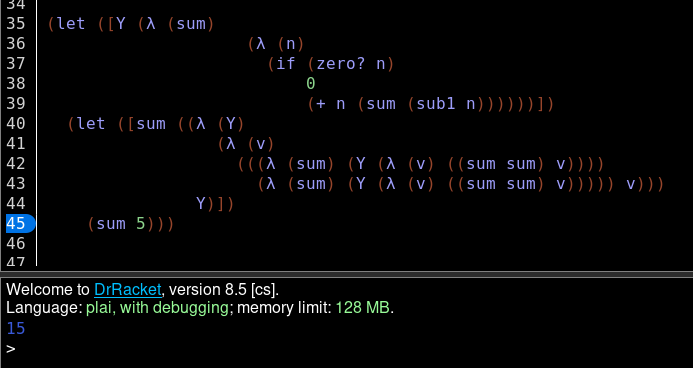
\includegraphics[scale=0.3]{./Sum-Y.png}
  \caption{Ejecución de la función dada.}
\end{figure}

Para esta función, tenemos una definición interna que realiza una recursión mutua,
la ejecución tiene que reducir las lambdas a su forma normal (en este caso siempre
es un valor numérico) y luego pasarselas a la función anterior o siguiente en el orden.
\newpage
%%%%%%%%%%%%%%%%%%%%%%%%%%%%%      Inciso C        %%%%%%%%%%%%%%%%%%%%%%%%%%%%%%%%%
\item Modifica la función usando el Combinador de Punto Fijo Z. Prueba la expresión en 
el intérprete de \code{Racket} y con base en la respuesta obtenida, explica el proceso que 
siguió el intérprete para llegar a ésta. Anexa una captura de pantalla del intérprete 
de \code{Racket} al probar la expresión.

\begin{figure}[h]
  \centering
  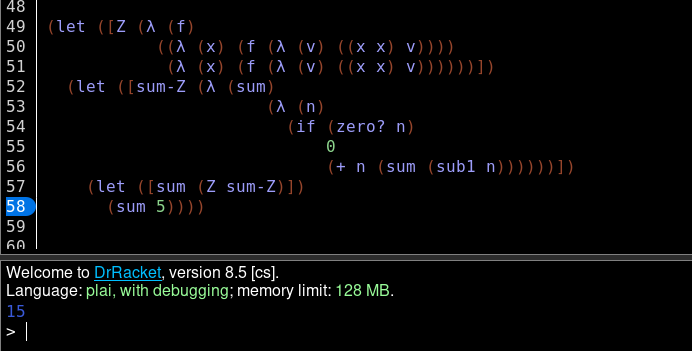
\includegraphics[scale=0.3]{./Sum-Z.png}
  \caption{Ejecución de la función dada.}
\end{figure}

Como en el ejercicio anterior, en la línea 27 se encuentra la modificación
que vuelve a esta función en un combinador de punto fijo Z. Inicialmente
reduce las lambdas a sus formas normales y ejecuta ambas funciones de manera
\textit{mutuamente recursiva} hasta llegar al valor deseado.
\end{enumerate}

	{\textcolor{blue}{6.}} Dada la siguiente expresión.
\begin{lstlisting}
    {with {w 2}
        {with {x 3}
            {with {y {+ w x } }
                {with { w -2}
                    {with {x -3 }
                        {+ y y } } } } } }
\end{lstlisting}
\begin{enumerate}
    \item[a.] Determinar el valor de la expresión. Muestra los pasos que hiciste para hacerlo.
    El proceso es el siguiente.

    Empezaremos con el primer with, podemos ver que la variable $w$ y se le asignará el valor de 2.
    \begin{lstlisting}
        {with {w 2}
    \end{lstlisting}

    Ahora pasamos al cuerpo del primer with. podemos ver que la variable $x$ todas las veces que salga en el cuerpo de
    este segundo with será sustituida por el valor de 3.

    \begin{lstlisting}
        {with {w 2}
            {with {x 3}
    \end{lstlisting}

    Ahora pasamos al cuerpo del segundo with (que es otro with). Podemos ver que la variable $y$ va a tener el valor de ${+ w x}$, pero los anteriores
    with ya nos dieron estos valores, por lo que nuestro valor para y es $\{+ \ 2 \ 3 \}$.

    \begin{lstlisting}
        {with {w 2}
            {with {x 3}
                {with {y {+ w x } }
    \end{lstlisting}

    Ahora pasamos al cuerpo del tercer with (que es otro with). aquí se nos vuelve a mostrar la variable $w$ sin embargo, todos los with dentro de este with
    tendrán en valor de la $w$ que se defina en este with, ya que opaca a las anteriores asignaciones. Por lo que el valor para esta $w$ es
    -2.

    \begin{lstlisting}
        {with {w 2}
            {with {x 3}
                {with {y {+ w x } }
                    {with { w -2}
    \end{lstlisting}

    Pasamos al cuerpo del cuarto with, que también es un with. Podemos ver que se vuelve a aplicar un valor a $x$, sin embargo sólo será tomado
    en cuenta para withs anidados dentro de este with. El valor para la $x$ es -2.

    \begin{lstlisting}
        {with {w 2}
            {with {x 3}
                {with {y {+ w x } }
                    {with { w -2}
                        {with {x -3 }
    \end{lstlisting}

    Finalmente llegamos al cuerpo del 5to with (el cual ya no es un with xd). Podemos ver que devuelve la operación $\{+ \ y \ y\}$. Sin embargo
    anteriormente ya habiamos obtenido el valor de $y$, el cual era $\{+ \ 2 \ 3\}$. por lo que lo sustituimos en $\{+ \ y \ y\}$ quedandonos
    $\{+ \ \{+ \ 2 \ 3\} \{+ \ 2 \ 3\}\}$.

    \begin{lstlisting}
        {with {w 2}
            {with {x 3}
                {with {y {+ w x } }
                    {with { w -2}
                        {with {x -3 }
                            {+ y y } } } } } }
    \end{lstlisting}

    Ahora evaluamos la operación resultante $\{+ \ \{+ \ 2 \ 3\} \{+ \ 2 \ 3\}\} = \{+ \ 5 \ 5\} = 10$

    \item[b.] ¿Pueden haber otros resultados? ¿Por qué?
    
    Sí, pueden haber otros resultados, esto debido a que depende del tipo de alcance que tienen los withs ya que existen 2 tipos, dinámico y estático.
    Dependiendo de cual se use, las variables se pueden buscar desde arriba, o el más cercano hacia abajo lo cual puede dar un resultado diferente en caso
    de que coloquemos id's iguales.
            
    \item[c.] ¿Cuál es el resultado correcto en dado caso de haber más de un posible resultado?
    
    Depende de la implementación de la función y del lenguaje de programación, pues si hay más de un resultado correcto es porque el lenguaje lo permite
    lo cual hace responsable al programador sobre el uso que requiera, o en otras palabras, el resultado correcto será aquel contemplado por el programador
    para realizar los calculos que requiere.
            
\end{enumerate}
\end{document}
